\documentclass[a4paper, titlepage]{article}
\usepackage[table]{xcolor}
\usepackage[T1]{fontenc}
\usepackage[utf8]{inputenc}
\usepackage[italian]{babel}
\usepackage{amsmath}
\usepackage{listings}
\usepackage{textcomp}
\usepackage{multirow}
\usepackage{multicol}
\usepackage{booktabs}
\usepackage{graphicx}
\usepackage{floatflt}
\usepackage{epsfig}
\usepackage{pstricks}
\usepackage{subfigure}
\usepackage[labelfont=bf, font=scriptsize]{caption}
\usepackage[italian]{varioref}
\usepackage[suftesi]{frontespizio}
\usepackage{color}
\usepackage{tikz}
\usepackage{caption}
\usepackage{comment}
\usepackage{lipsum}
\usepackage{hyperref}
\usepackage{graphicx}
\usepackage[margin=2cm]{geometry}
%\usepackage{pgfplots}
\usepackage{comment}
\usepackage{lipsum}
\usepackage{longtable}
%\pgfplotsset{compat=1.16}

%%% Il documento vero e proprio %%%
\begin{document}

%%% Frontespizio %%%
\begin{frontespizio}
\Universita{Padova} 
\Logo{Fig/logo_unipd} 
\Dipartimento{Matematica}
\Corso[Laurea Magistrale]{Informatica} 

\Annoaccademico{2020-2021}
\Titoletto{Algoritmi Avanzati \\ Relazione di laboratorio 1}
\Titolo{Minimum Spanning Tree}
\Sottotitolo{Aprile 2021}
\NCandidati{Gruppo di lavoro} 
\Candidato[2029254]{Sofia Bononi}
\Candidato[2022146]{Davide Franzoso}
\Candidato[2029214]{Matteo Mariani}
\end{frontespizio}

%%% Indice %%%
\tableofcontents

\newpage
%%% Sezioni %%%
\section{Introduzione}
\label{Introduzione}

In questa relazione viene descritta l'implementazione e lo studio delle performance di tre algoritmi \texttt{Prim, Kruskal naive e Kruskal con implementazione Union-Find} i quali prendono in input un grafo non diretto, connesso e pesato, e come output restituiscono il minimum spanning tree che tocca tutti i nodi del grafo e che minimizza la somma totale dei pesi di tutti i lati dell'albero.
Per ciascun algoritmo verrà riportata la nostra implementazione e i corrispondenti risultati ottenuti.

\section{Classi}
\label{Classi}

Per implementare gli algoritmi sono state create 4 classi di oggetti, una classe di Utility e un Main.

\subsection{Arco}
\label{Arco}

L'oggetto \textit{Arco} contiene le infomazioni relative ad un arco:

\begin{itemize}
    \item \textbf{nodo1}: nodo iniziale;
    \item \textbf{nodo2}: nodo finale;
    \item \textbf{peso}: peso dell'arco;
    \item \textsc{getArco()}: funzione che restituisce una lista [nodo1, nodo2, peso]
    \item \textsc{getArcoInverso()}: funzione che, chiamata su un arco \emph{(u,v)} , ne restituisce l'inverso \emph{(v,u)}
\end{itemize}

\subsection{Grafo}
\label{Grafo}

L'oggetto \textit{Grafo} contiene le informazioni relative ad un grafo:

\begin{itemize}
    \item \textbf{n\_nodi}: campo dati che indica il numero dei nodi;
    \item \textbf{n\_archi}: campo dati che indica il numero degli archi;
    \item \textbf{lista\_nodi}: campo dati che contiene un insieme set() di nodi; 
    \item \textbf{lista\_archi}: campo dati che contiene la lista di oggetti arco;
    \item \textbf{id2Node}: Dizionario avente come campo key l'identificatore di un nodo (intero) e come valore l'oggetto nodo corrispondente a quell'identificativo;
    \item \textbf{lista\_adiacenza}:Dizionario avente come campo key l'intero corrispondente ad un nodo,  e come valore la lista di archi adiacenti al nodo;
    \item \textbf{lista\_adiacenza\_nodi}: Dizionario avente come campo key l'intero corrispondente ad un nodo,  e come valore la lista di oggetti nodi adiacenti al nodo;
    \item \textbf{totPeso}: campo dati che indica il peso totale degli archi del grafo, calcolato da uno degli algoritmi presentati;
    \item \textsc{aggiungiArco(arco)}: metodo che dato in input un arco lo aggiunge agli archi del grafo;
    \item \textsc{getNodo(id\_nodo)}: metodo che dato in input l'id di un nodo restituisce l'oggetto del nodo corrispondente;
    \item \textsc{getListaNodi()}: metodo che restituisce la lista di  oggetti nodi;
    \item \textsc{getGrafoPrim()}: metodo che, utilizzando le relazioni padre-figlio risultanti dall'algoritmo Prim, restituisce un nuovo grafo basato su tali relazioni (utile per i test).
\end{itemize}

\subsection{Nodo}
\label{Nodo}

L'oggetto \textit{Nodo} contiene le informazioni relative ad un nodo:

\begin{itemize}
    \item \textbf{nodo}: Intero identificativo del nodo;
    \item \textbf{padre}: Intero che identifica il padre v di un nodo u nell'albero di copertura minimo;
    \item \textbf{key}: Campo utilizzato per costruire il min heap, inizializzato con il peso dell'arco adiacente al nodo. Ad esempio il campo key del nodo \emph{u} sarà inizializzato con il valore \emph{w(u,v)};
    \item \textbf{in\_h}: Intero per verificare se un nodo è stato estratto dall'heap o meno;
    \item \textbf{vis}: Intero per verificare se un nodo è stato visitato o meno nella procedura dfs
    \item \textbf{heapIndex}:Indice utilizzato per tenere traccia della posizione di ogni nodo all'interno dell'heap
\end{itemize}

\subsection{Utility}
\label{Utility}

La classe \textit{Utility} contiene le funzioni che ci sono servite per implementare i tre algoritmi. 

\begin{itemize}
    \item \textsc{inizializzaGrafo(n\_g, g)}: metodo che prende in input un grafo \textsc{g} ed inizializza il grafo \textsc{n\_g} con gli stessi nodi.
\end{itemize} 

All'interno di questa classe troviamo tre metodi che sono stati utilizzati per implementare \textsc{Kruskal - Union-Find}, in particolare:
\begin{itemize}
    \item \textsc{MakeSet(nodo)}: metodo che prende in input un nodo e lo inizializza come padre di sé stesso;
    \item \textsc{Union(nodo1, nodo2, g)}: metodo che prende in input due nodi e un grafo e, se questi due nodi fanno parte di due insiemi disguinti diversi, unisce le componenti connesse che li contengono, facendo puntare la radice dell'albero con profondità minima a quella del secondo albero, minimizzando quindi la profondità totale;
    \item \textsc{FindSet(g, nodo1)}: metodo che ritorna la radice dell'insieme in cui è contenuto il nodo1 passato in input, risalendo di padre in padre fino a trovare un self-loop (ossia un elemento che punta a sé stesso). 
\end{itemize}

\newpage

\subsection{Heap}
\label{Heap}

L'oggetto \textit{Heap} contiene le funzioni che permettono di realizzare un \textit{min-heap}. Uno heap è una struttura dati che si può considerare un albero binario quasi completo, ovvero un albero nel quale tutti i livelli sono riempiti quasi completamente tranne l'ultimo. Le caratteristiche dello heap sono:

\begin{itemize}
    \item l'ultimo livello incompleto si riempie da sinistra;
    \item l'albero viene rappresentato sotto forma di array A che è caratterizzato da \textit{A.length} che rappresenta la lunghezza di A e \textit{A.heapsize} che rappresenta la dimensione dello heap.
\end{itemize}

Per implementare l'algoritmo è stato realizzato un \textit{min-heap}, uno heap caratterizzato da nodi con la chiave minore o uguale a quella dei figli. Quindi la radice rappresenta l'elemento più piccolo del \textit{min-heap}.

L'oggetto \textit{Nodo} contiene:

\begin{itemize}
    \item \textbf{vector}: vettore associato allo heap;
    \item \textbf{length}: lunghezza del vettore;
    \item \textbf{heapsize}: lunghezza dello heap;
    \item \textsc{BuildMinHeap(h)}: metodo che dato in input l'oggetto heap, costruisce un \textit{min-heap};
    \item \textsc{MinHeapify(h, i)}: metodo che dato in input un vettore e un nodo, sistema il nodo nella posizione corretta;
    \item \textsc{HeapDecreaseKey(h, i ,key)}: metodo che dato in input uno heap, un indice ed una nuova chiave, sostituisce il valore del vettore associato all'indice i con il nuovo valore key;
    \item \textsc{HeapMinimum(h)}: metodo che dato in input un heap, restituisce il valore minimo dello heap, ossia la radice;
    \item \textsc{HeapExtractMin(h)}: metodo che dato in input un heap, trova l'elemento più piccolo, lo rimuove e ritorna l'oggetto;
    \item \textsc{isIn(h, v)}:
    \item \textsc{right(index)}: metodo che, dato in input un indice di un nodo, restituisce l'indice del nodo figlio destro;
    \item \textsc{left(index)}: metodo che, dato in input un indice di un nodo, restituisce l'indice del nodo figlio sinistro;
    \item \textsc{parent(index)}:metodo che, dato in input un indice di un nodo, restituisce l'indice del padre;
\end{itemize}


\newpage

\subsection{Main}
\label{Main}

La classe \textit{Main} contiene il dataset dei grafi dopo l'esecuzione del parsing, le funzioni di parsing, di misurazione di performance e le implementazioni degli algoritmi:

\begin{itemize}
    \item \textsc{parsing(directory)}: funzione che, data in input una directory, analizza tutti i file interni e seleziona solo quelli con estensione .txt, fornendoli in input alla funzione crea\_grafi();
    \item \textsc{crea\_grafi(file)}: funzione che, dato in input un file, lo legge ed estrae le informazioni per la creazione di oggetti Grafo, Nodo e Arco;
    \item \textsc{plot\_graph()}: plot\_graph è una funzione che viene utilizzata per creare i grafici delle performance degli algoritmi utilizzati ;
    
    \item \textsc{measurePerformance()}:measurePerformance() è la funzione che viene utilizzata per calcolare tutte quelle metriche utili per valutare le performance di un algoritmo e per creare il successivo grafico. Le metriche calcolate sono:
    \begin{itemize}
        \item  totTimes:  totTimes è una matrice avente di dimensionalità $mxn$ dove m è uguale al numero di algoritmi testati mentre n è il numero di dimensionalità di grafi considerati.
        \item totRatios: totRatios è una matrice della stessa dimensionlità di totTimes contenente tutti i ratio tra il tempo di calcolo medio tra le istanze di dimensionalità $n$ e il tempo di calcolo medio tra le istante di dimensionalità $m$ tale che $m>n$
        \item  totConstant:  totConstant è una matrice contenente le costanti nascoste per ogni algoritmo e per ogni dimensionalità di input considerata
    \end{itemize};
    \item \textsc{measure\_run\_time(n\_instances, graphs, algorithm)}: measure\_run\_time è la funzione chiamata da  measurePerformance() per calcolare i tempi per ciascun algoritmo. Per aumentare l'affidabilità delle misurazioni per istanze di bassa dimensionalità (numero di nodi <= 100) gli algoritmi sono stati ripetuti più volte (30) e poi il tempo è stato calcolato dividendo il tempo totale per questo numero di iterazioni. Per ottenere un ulteriore grado di accuratezza sulle misurazioni sono state testati 4 input della stessa dimensionalità $n$ per ogni $n$ e anche qui poi è stata presa la media.;
    
    \item \textsc{plot\_graph())}: .
\end{itemize}


\newpage
\newpage
\section{Classi}
\label{Classi}

Per implementare gli algoritmi sono state create 4 classi di oggetti, una classe di Utility e un Main.

\subsection{Arco}
\label{Arco}

L'oggetto \textit{Arco} contiene le infomazioni relative ad un arco:

\begin{itemize}
    \item \textbf{nodo1}: nodo iniziale;
    \item \textbf{nodo2}: nodo finale;
    \item \textbf{peso}: peso dell'arco;
    \item \hypertarget{getarco}{\textsc{getArco()}}: funzione che restituisce una lista [nodo1, nodo2, peso]
    \item \hypertarget{getarcoinverso}{\textsc{getArcoInverso()}}: funzione che, chiamata su un arco \emph{(u,v)} , ne restituisce l'inverso \emph{(v,u)}
\end{itemize}

%%%%%%%%%%%%%%%%%%%%%%%%%%%%%%%%%%%%%%%%%%%%%%%%%%%%%%%%%%%%%%%%%%%%%%%%%%%%%%%%%%%%%%%%%%%%%%%%%%%%%%%%%

\subsection{Grafo}
\label{Grafo}

L'oggetto \textit{Grafo} contiene le informazioni relative ad un grafo:

\begin{itemize}
    \item \textbf{n\_nodi}: campo dati che indica il numero dei nodi;
    \item \textbf{n\_archi}: campo dati che indica il numero degli archi;
    \item \textbf{lista\_nodi}: campo dati che contiene un insieme set() di nodi; 
    \item \textbf{lista\_archi}: campo dati che contiene la lista di oggetti arco;
    \item \textbf{id2Node}: Dizionario avente come campo key l'identificatore di un nodo (intero) e come valore l'oggetto nodo corrispondente a quell'identificativo;
    \item \textbf{lista\_adiacenza}:Dizionario avente come campo key l'intero corrispondente ad un nodo,  e come valore la lista di archi adiacenti al nodo;
    \item \textbf{lista\_adiacenza\_nodi}: Dizionario avente come campo key l'intero corrispondente ad un nodo,  e come valore la lista di oggetti nodi adiacenti al nodo;
    \item \textbf{totPeso}: campo dati che indica il peso totale degli archi del grafo, calcolato da uno degli algoritmi presentati;
    \item \hypertarget{aggiungiarco}{\textsc{aggiungiArco(arco)}}: metodo che dato in input un arco lo aggiunge agli archi del grafo;
    \item \hypertarget{getnodo}{\textsc{getNodo(id\_nodo)}}: metodo che dato in input l'id di un nodo restituisce l'oggetto del nodo corrispondente;
    \item \hypertarget{getlistanodi}{\textsc{getListaNodi()}}: metodo che restituisce la lista di  oggetti nodi;
    \item \hypertarget{getgrafoprim}{\textsc{getGrafoPrim()}}: metodo che, utilizzando le relazioni padre-figlio risultanti dall'algoritmo Prim, restituisce un nuovo grafo basato su tali relazioni (utile per i test).
\end{itemize}

%%%%%%%%%%%%%%%%%%%%%%%%%%%%%%%%%%%%%%%%%%%%%%%%%%%%%%%%%%%%%%%%%%%%%%%%%%%%%%%%%%%%%%%%%%%%%%%%%%%%%%%%%

\subsection{Nodo}
\label{Nodo}

L'oggetto \textit{Nodo} contiene le informazioni relative ad un nodo:

\begin{itemize}
    \item \textbf{nodo}: Intero identificativo del nodo;
    \item \textbf{padre}: Intero che identifica il padre v di un nodo u nell'albero di copertura minimo;
    \item \textbf{key}: Campo utilizzato per costruire il min heap, inizializzato con il peso dell'arco adiacente al nodo. Ad esempio il campo key del nodo \emph{u} sarà inizializzato con il valore \emph{w(u,v)};
    \item \hypertarget{inh}{\textbf{in\_h}}: Intero per verificare se un nodo è stato estratto dall'heap o meno;
    \item \textbf{vis}: Intero per verificare se un nodo è stato visitato o meno nella procedura dfs
    \item \textbf{heapIndex}:Indice utilizzato per tenere traccia della posizione di ogni nodo all'interno dell'heap
\end{itemize}

%%%%%%%%%%%%%%%%%%%%%%%%%%%%%%%%%%%%%%%%%%%%%%%%%%%%%%%%%%%%%%%%%%%%%%%%%%%%%%%%%%%%%%%%%%%%%%%%%%%%%%%%%

\subsection{Utility}
\label{Utility}

La classe \textit{Utility} contiene le funzioni di servizio per implementare i tre algoritmi. In questa classe sono state aggiunte anche le funzioni necessarie per costruire la struttura dati UnionFind e alcune funzioni utili per le prove di correttezza dei risultati.

\begin{itemize}
    
    \item \hypertarget{inizializzagrafo}{\textbf{\textsc{inizializzaGrafo(n\_g, g)}}}: metodo che prende in input un grafo \textsc{g} ed inizializza il grafo \textsc{n\_g} con gli stessi nodi.
    
    \item \hypertarget{merge}{\textbf{\textbf{\textsc{merge(array, p, q, r)}}}}: metodo che implementa l'algoritmo merge modificato per confrontare i pesi degli archi. Data una lista archi, p, q, r sono indici dell'array, tali che \texttt{p <= q < r}. Gli indici dividono l'array in sottosequenze: \texttt{A[p..q] A[q+1..r]};
    
    \item \hypertarget{mergesort}{\textbf{\textsc{mergeSort\_weight(array, p, r)}}}: metodo che implementa l'algortimo di ordinamento mergeSort;
    
    \item \hypertarget{dfsciclo}{\textbf{\textsc{dfs\_ciclo(g, u, padri, visitati)}}}: metodo utilizzato per la ricerca di cicli nell'algoritmo \hyperlink{section.4}{\textsc{Kruskal-naive}}. La funzione prende in input un grafo da analizzare, un nodo di partenza, un vettore dei padri e un vettore dei visitati (inizializzati a 0). Viene eseguita una visita DFS de grafo e ad ogni iterazione viene visitato un nodo e ricorsivamente tutti i suoi vicini impostando ad 1 il vettore dei visitati e costruendo il vettore dei padri, se si incontra un nodo già visitato (ad eccezione del padre) la funzione restituisce True, poichè è stato trovato un ciclo nel grafo.
    
    \item \hypertarget{dfssupporto}{\textbf{\textsc{dfs\_supporto(g, u, n\_nodi, visitati)}}}: 
    
    \item \hypertarget{testalberosupporto}{\textbf{\textsc{test\_albero\_supporto(lista\_grafi)}}}: 
    
    
\end{itemize} 

Seguono i metodi utilizzati per implementare \textsc{Kruskal-UnionFind}:
\begin{itemize}
    \item \hypertarget{makeset}{\textbf{\textsc{MakeSet(nodo)}}}: metodo che prende in input un nodo e lo inizializza come padre di sé stesso;
    
    \item \hypertarget{union}{\textbf{\textsc{Union(nodo1, nodo2, g)}}}: metodo che prende in input due nodi e un grafo e, se questi due nodi fanno parte di due insiemi disguinti diversi, unisce le componenti connesse che li contengono, facendo puntare la radice dell'albero con profondità minima a quella del secondo albero, minimizzando quindi la profondità totale;
    
    \item \hypertarget{findset}{\textbf{\textsc{FindSet(g, nodo1)}}}: metodo che ritorna la radice dell'insieme in cui è contenuto il nodo1 passato in input, risalendo di padre in padre fino a trovare un self-loop (ossia un elemento che punta a sé stesso).
\end{itemize}

\newpage

%%%%%%%%%%%%%%%%%%%%%%%%%%%%%%%%%%%%%%%%%%%%%%%%%%%%%%%%%%%%%%%%%%%%%%%%%%%%%%%%%%%%%%%%%%%%%%%%%%%%%%%%%

\subsection{Heap}
\label{Heap}

L'oggetto \textit{Heap} contiene le funzioni che permettono di realizzare un \textit{min-heap}. Uno heap è una struttura dati che si può considerare un albero binario quasi completo, ovvero un albero nel quale tutti i livelli sono riempiti quasi completamente tranne l'ultimo. Le caratteristiche dello heap sono:

\begin{itemize}
    \item l'ultimo livello incompleto si riempie da sinistra;
    \item l'albero viene rappresentato sotto forma di array A che è caratterizzato da \textit{A.length} che rappresenta la lunghezza di A e \textit{A.heapsize} che rappresenta la dimensione dello heap.
\end{itemize}


Per implementare l'algoritmo è stato realizzato un \textit{min-heap}, uno heap caratterizzato da nodi con la chiave minore o uguale a quella dei figli. Quindi la radice rappresenta l'elemento più piccolo del \textit{min-heap}.


\begin{itemize}
    \item \textbf{vector}: vettore associato allo heap;
    \item \textbf{length}: lunghezza del vettore;
    \item \textbf{heapsize}: lunghezza dello heap;
    \item \hypertarget{buildminheap}{\textsc{BuildMinHeap(h)}}: metodo che dato in input l'oggetto heap, costruisce un \textit{min-heap};
    \item \hypertarget{minheapify}{\textsc{MinHeapify(h, i)}}: metodo che dato in input un vettore e un nodo, sistema il nodo nella posizione corretta;
    \item \hypertarget{heapdecreasekey}{\textsc{HeapDecreaseKey(h, i ,key)}}: metodo che dato in input uno heap, un indice ed una nuova chiave, sostituisce il valore del vettore associato all'indice i con il nuovo valore key;
    \item \hypertarget{heapminimum}{\textsc{HeapMinimum(h)}}: metodo che dato in input un heap, restituisce il valore minimo dello heap, ossia la radice;
    \item \hypertarget{heapextractmin}{\textsc{HeapExtractMin(h)}}: metodo che dato in input un heap, trova l'elemento più piccolo, lo rimuove e ritorna l'oggetto;
    \item \hypertarget{isin}{\textsc{isIn(h, v)}}: metodo che, dato in input un nodo, restituisce 1 se esso è presente nell'heap, 0 altrimenti. Per rendere questa operazione di tempo costante è stata aggiunto un attributo \hyperlink{inh}{\textit{in\_h}} ad ogni nodo.
    \item \hypertarget{right}{\textsc{right(index)}}: metodo che, dato in input un indice di un nodo, restituisce l'indice del nodo figlio destro;
    \item \hypertarget{left}{\textsc{left(index)}}: metodo che, dato in input un indice di un nodo, restituisce l'indice del nodo figlio sinistro;
    \item \hypertarget{parent}{\textsc{parent(index)}}:metodo che, dato in input un indice di un nodo, restituisce l'indice del padre;
\end{itemize}


\newpage

%%%%%%%%%%%%%%%%%%%%%%%%%%%%%%%%%%%%%%%%%%%%%%%%%%%%%%%%%%%%%%%%%%%%%%%%%%%%%%%%%%%%%%%%%%%%%%%%%%%%%%%%%

\subsection{Main}
\label{Main}

La classe \textit{Main} contiene il dataset dei grafi dopo l'esecuzione del parsing, le funzioni di parsing, di misurazione di performance e le implementazioni degli algoritmi:

\begin{itemize}
    
    \item \textbf{lista\_grafi}: vettore utilizzato per la memorizzazione dei grafi dopo l'esecuzione del \hyperlink{parsing}{parsing};
    
    \item \textbf{p\_g}: vettore contenente i grafi risultanti dall'esecuzione dell'algoritmo \texttt{Prim};
    
    \item \textbf{k\_g}: vettore contenente i grafi risultanti dall'esecuzione dell'algoritmo \texttt{Kruskal-UnionFind};
    
    \item \textbf{kn\_g}: vettore contenente i grafi risultanti dall'esecuzione dell'algoritmo \texttt{Kruskal-Naive};
    
    
    \item \hypertarget{parsing}{\textsc{parsing(directory)}}: funzione che, data in input una directory, analizza tutti i file interni e seleziona solo quelli con estensione .txt, fornendoli in input alla funzione \hyperlink{creagrafi}{crea\_grafi()};
    
    \item \hypertarget{creagrafi}{\textsc{crea\_grafi(file)}}: funzione che, dato in input un file, lo legge ed estrae le informazioni per la creazione di oggetti Grafo, Nodo e Arco;
    
    \item \hypertarget{plotgrafi}{\textsc{plot\_graph()}}: plot\_graph è una funzione che viene utilizzata per creare i grafici delle performance degli algoritmi utilizzati ;
    
    \item \hypertarget{measureperformance}{\textsc{measurePerformance()}}:measurePerformance() è la funzione che viene utilizzata per calcolare tutte quelle metriche utili per valutare le performance di un algoritmo e per creare il successivo grafico. Le metriche calcolate sono:
   
    \begin{itemize}
        
        \item  \textbf{totTimes}:  totTimes è una matrice avente di dimensionalità $mxn$ dove m è uguale al numero di algoritmi testati mentre n è il numero di dimensionalità di grafi considerati.
        
        \item\textbf{totRatios}: totRatios è una matrice della stessa dimensionlità di totTimes contenente tutti i ratio tra il tempo di calcolo medio tra le istanze di dimensionalità $n$ e il tempo di calcolo medio tra le istante di dimensionalità $m$ tale che $m>n$
        
        \item  \textbf{totConstant}:  totConstant è una matrice contenente le costanti nascoste per ogni algoritmo e per ogni dimensionalità di input considerata
    \end{itemize};
    
    \item \hypertarget{measureruntime}{\textsc{measure\_run\_time(n\_instances, graphs, algorithm)}}: measure\_run\_time è la funzione chiamata da  measurePerformance() per calcolare i tempi di esecuzione di ciascun algoritmo. Per aumentare l'affidabilità delle misurazioni per istanze di bassa dimensionalità (numero di nodi <= 100) gli algoritmi sono stati ripetuti più volte (30) e poi il tempo è stato calcolato dividendo il tempo totale per questo numero di iterazioni. Per ottenere un ulteriore grado di accuratezza sulle misurazioni sono state testati 4 input della stessa dimensionalità $n$ per ogni $n$ e anche qui poi è stata presa la media.;
\end{itemize}


\newpage
\newpage
\section{Algoritmo di Prim}
\label{Prim}

L'algoritmo di Prim, dato un grafo G = (V,E) ed un nodo di partenza s, costruisce un MST, partendo da un albero A (con un singolo nodo) e aggiungendo, ad ogni passo, un light edge a lui collegato che sia sicuro\footnote{Un lato si dice sicuro se, la sua aggiunta, conserva l'invariante per cui: prima di ogni iterazione, A è un sottoinsieme di qualche albero di connessione minimo.} per A.

\subsection{Strutture dati}
\label{strutture_dati}

Le strutture dati utilizzate per implementare questo algoritmo sono:

\begin{itemize}
    \item classe Grafo;
    \item classe Nodo;
    \item classe Heap:
    \begin{itemize}
        \item metodo BuildMinHeap(h);
        \item metodo isIn(v);
        \item metodo HeapDecreaseKey(h, i, key).
    \end{itemize}
\end{itemize}

La descrizione si piò trovare alla sezione \textsc{1.2 Classi}.

\subsection{Implementazione}
\label{implementazione}

Questo algoritmo è stato implementato nel seguente modo:

\begin{itemize}
    \item è stata inizializzata la lista di nodi;
    \item al campo key di ogni nodo è stato assegnato il valore infinito;
    \item al campo key del nodo radice, dato in input, è stato assegnato il valore 0;
    \item è stata inizializzata una struttura heap a cui è stato passato come paramentro la lista dei nodi del grafo \texttt{g} dato in input;
    \item utilizzando il metodo \hyperlink{buildminheap}{\textsc{BuildMinHeap()}} è stato realizzato un min-heap;
    \item viene iterato lo heap e, grazie al metodo \hyperlink{heapextractmin}{\textsc{HeapExtractMin()}} , viene estratto il nodo con campo key minimo;
    \item viene salvato il suo valore key in modo da salvare il peso totale dell'albero una volta terminato l'algoritmo;
    \item per ogni arco nella lista di adiacenza del nodo estratto  viene controllato se il nodo adiacente è nell heap e se il peso dell'arco tra i due è minore del valore del campo key del nodo considerato. Se il risultato è positivo si procede con l'aggiornamento dei campi, utilizzando \hyperlink{heapdecreasekey}{\textsc{HeapDecreaseKey()}}.

Dato che \textsc{HeapDecreaseKey()} richiede in input la posizione del nodo che si vuole aggiornare, la prima implementazione è stata utilizzando la funzione python index() ma, andando ad analizzare successivamente la complessità di Prim essa non corrispondeva alla complessità teorica di $O(m log{} n)$. Quindi è stato aggiundo un ulteriore campo \textsc{heapIndex} alla classe node per tenere traccia degli indici dei nodi all'interno dell heap e riducendo così la complessità di recucpero dell'indice da $O(n)$ a $O(1)$.

\end{itemize}
	
\newpage
\section{Algoritmo di Kruskal -- Naive}
\label{Algoritmo_di_Kruskal-naive}

L'algoritmo Kruskal--Naive è una prima implementazione dell'algoritmo di Kruskal per l'individuazione di un albero di copertura minimio. Come si vedrà in seguito, è possibile migliorare notevolmente questo algoritmo grazie all'utilizzo di una particolare struttura dati per l'individuazione di cicli nel grafo. L'idea alla base di questa implementazione consiste nel costruire il MST aggiungendo, ad ogni iterazione, l'arco con peso minimo e controllando che esso non porti alla formazione di cicli nel grafo. 

\subsection{Strutture dati}
\label{strutture_dati}

Le strutture dati utilizzate per implementare questo algoritmo sono:

\begin{itemize}
    \item classe Grafo;
    \item classe Arco;
    \item metodo \hyperlink{inizializzagrafo}{inizializzaGrafo(n\_g, g)};
    \item metodo \hyperlink{mergesort}{mergeSort\_weight(array, p, r)};
    \item metodo \hyperlink{dfsciclo}{dfs\_ciclo(g, u, padri, visitati)}.
\end{itemize}

Per la descrizione delle classi si rimanda alla sezione \hyperlink{section.2}{1.2 Classi}.
\newline

\subsection{Implementazione}
\label{implementazione}

L'algoritmo è stato implementato nel seguente modo:
\begin{itemize}
    
    \item vengono creati due oggetti grafo, uno sarà il grafo MST e l'altro un grafo fittizio utile per verificare la presenza di cicli in tempi ridotti;
    
    \item viene eseguito il mergeSort per ordinare gli archi rispetto al peso;
    
    \item vengono inizializzati i due grafi con tutti i nodi del grafo in input (è chiaro, infatti, che i nodi devono essere gli stessi del grafo in input ed aggiungerli ad ogni passo sarebbe solo una superflua complicazione);
    
    \item si scorre quindi la lista di archi ordinati e, ad ogni iterazione, viene aggiornata la lista di adiacenza del grafo fittizio con l'aggiunta dell'arco selezionato (si noti che la lista di adiacenza è l'unico parametro del grafo di cui si ha bisogno per eseguire la \hyperlink{dfsciclo}{dfs\_ciclo()}, o una qualsiasi dfs);
    
    \item a questo punto, con la lista di adiacenza aggiornata vengono inizializzati a 0 il vettore dei visitati e dei padri in quanto ad ogni esecuzione della \hyperlink{dfsciclo}{dfs\_ciclo()} è necessario che questi siano indipendenti dalla visita precedente, altrimenti avremmo nodi già visitati e cicli inesistenti;
    
    \item se non viene trovato alcun ciclo si procede con l'aggiunta dell'arco e delle rispettive dipendenze (numero archi, lista di adiacenza , ecc..) al grafo MST;
    
    \item se, invece, viene trovato un ciclo, si esegue un pop() dalla lista di adiacenza del grafo fittizio (è possibile eseguire questa operazione, di costo O(1), poiché l'unica aggiunta che era stata fatta sul grafo fittizio consisteva di un append() sulla lista di adiacenza);
    
    \item per velocizzare ulteriormente i tempi, si è pensato inoltre di non eseguire l'algoritmo per ogni arco del grafo, bensì di fermarsi una volta raggiunti (dato n il numero dei nodi) gli n-1 archi.
    
\end{itemize}

\newpage
\section{Algoritmo di Kruskal -- Union-Find}
\label{Algoritmo_di_Kruskal_Union-Find}

L'algoritmo di Kruskal permette di costruire, dato un qualsiasi grafo pesato e non diretto, un albero di copertura minimo (MST), aggiungendo ad ogni iterazione un nuovo arco (di peso minimo) all'insieme grafo e controllando, utilizzando la struttura dati \textit{Union-Find}, che esso non crei cicli. \\
La struttura dati \textit{Union-Find} gestisce insiemi disgiunti di oggetti, ciò significa che un oggetto può stare in uno e uno solo dei sottoinsiemi degli insiemi disgiunti presenti nella \textit{Union-Find}.

\subsection{Strutture dati}
\label{strutture_dati}

Le strutture dati e i metodi utilizzati per implementare questo algoritmo sono:

\begin{itemize}
    \item classe Grafo;
    \item classe Arco;
    \item metodo inizializzaGrafo(n\_g, g);
    \item metodo \hyperlink{makeset}{MakeSet(nodo)};
    \item metodo MergeSort\_weight(array, p, r);
    \item metodo \hyperlink{findset}FindSet(nodo1, nodo2, g);
    \item metodo \hyperlink{union}Union(g, nodo1).
\end{itemize}

Per la descrizione delle classi si rimanda alla sezione \hyperlink{section.2}{1.2 Classi}.
\newline
Per la descrizione dei metodi si rimanda alla sezione \hyperlink{subsection.2.4}{2.4 Utility}

\subsection{Implementazione}
\label{implementazione}

L'algoritmo è implementato nel seguente modo:

\begin{itemize}
    \item viene definito un grafo \texttt{grafo} e inizializzato con gli stessi nodi del grafo \texttt{g} dato in input.
    \item attraverso l'operazione MakeSet viene creato un albero per ogni nodo del grafo;
    \item utilizzando l'algoritmo di MergeSort\_weight viene ordinata la lista degli archi del grafo in maniera crescente rispetto al peso;
    \item per ogni arco si controlla, risalendo alla radice (attraverso la funzione FindSet(nodo)), se gli insiemi dei suoi nodi coincidono. Se le radici dei nodi sono diverse si giunge alla conclusione che le due componenti sono distinte e quindi l'arco può essere aggiunto al grafo \texttt{grafo}, in quanto non crea un ciclo. 
    \item nel caso in cui l'arco venga aggiungo al grafo \texttt{grafo}, si aggiornano gli insiemi attraverso l'operazione di union.
\end{itemize}


\subsection{Complessità}
\label{complessità}
\newpage
\section{Correttezza}
\label{correttezza}

Complementari all'implmentaione di un algoritmo sono le prove di correttezza che vengono fornite per sancirne la bontà. Nel caso degli algoritmi di \texttt{Prim, Kruskal e Kruskal-naive}, abbiamo ritenuto opportuno verificare le seguenti ipotesi:

\begin{itemize}
    
    \item che i grafi risultanti dai 3 algoritmi avessero rispettivamente \textbf{stesso peso};
    
    \item che i grafi risultanti dai 3 algoritmi fossero tutti degli \textbf{alberi di supporto}.

\end{itemize}

\subsection{Correttezza Pesi}
\label{correttezza_pesi}
Per provare la correttezza dei pesi calcolati si è pensato di eseguire un semplice controllo di uguaglianza tra i pesi dei grafi MST calcolati dai 3 algoritmi.

\begin{itemize}
    \item \textbf{test\_tot\_pesi(prim, kruskal, kruskal\_naive)}: scorrendo l'array dei grafi risultanti dall'esecuzione degli algoritmi, viene eseguito il confronto tra i pesi, utilizzando l'attributo \texttt{totPeso} di ogni \hyperlink{subsection.2.2}{oggetto grafo}.
\end{itemize}

\subsection{Alberi di supporto}
\label{alberi_supporto}

Per dimostrare la correttezza delle strutture grafi ottenuti si è dimostrato che ogni grafo MST risultante fosse un albero di supporto, per fare ciò, sono state verificate due condizioni, in ogni grafo:

\begin{itemize}
    \item tutti i nodi del grafo sono connessi;
    \item dati n nodi il grafo possiede n-1 archi;
\end{itemize}

A questo proposito sono stati sviluppati tre algoritmi:

\begin{itemize}
    \item \textbf{dfs\_supporto(g, u, n\_nodi, visitati)}: viene eseguita una visita dfs del grafo e riempita una lista per verificare se tutti i nodi vengono visitati;
    
    \item \textbf{test\_albero\_supporto(lista\_grafi)}: viene eseguita dfs\_supporto() per ogni grafo risultante da uno dei 3 algoritmi, per ognuno di essi viene controllato che i nodi visitati siano tutti i nodi del grafo e che, dato n il numero dei nodi, gli archi siano n-1;
    
    \item \textbf{test\_total\_supporto(prim, kruskal\_naive, kruskal)}: viene eseguito test\_albero\_supporto() per i grafi risultanti da tutti e tre gli algoritmi e viene restituito un messaggio a schermo per comunicare il risultato dei test.
    
    
\end{itemize}

\newpage

Di seguito un esempio dell'output di test\_total\_supporto(prim, kruskal\_naive, kruskal):

--------------------

Numero di nodi nel grafo:  10 

Numero di nodi visitati con dfs:  10

Numero di archi nel grafo:  9

É un albero di supporto?:  True

Peso totale dell'albero:  29316

--------------------

Numero di nodi nel grafo:  10

Numero di nodi visitati con dfs:  10

Numero di archi nel grafo:  9

É un albero di supporto?:  True

Peso totale dell'albero:  25217

--------------------

Numero di nodi nel grafo:  10

Numero di nodi visitati con dfs:  10

Numero di archi nel grafo:  9

É un albero di supporto?:  True

Peso totale dell'albero:  16940

--------------------

Numero di nodi nel grafo:  10

Numero di nodi visitati con dfs:  10

Numero di archi nel grafo:  9

É un albero di supporto?:  True

Peso totale dell'albero:  -44448

--------------------
\newline \\
I risultati dei test eseguiti restituiscono tutti esiti positivi.

    


\newpage
\section{Performance}
Abbiamo misurato le performance (in millisecondi) dei tre algoritmi utilizzando 68 grafi di diverse dimensioni.
I grafi testati hanno un numero di nodi che variavano dai  10 ai 100000.
Come già detto, per ogni dimensione sono presenti quattro grafi e, per ottenere una misurazione dei tempi più precisa, vengono calcolati e sommati i tempi per ogni grafo (della stessa dimensionalità) e il tempo medio viene calcolato dividendo questo risultato per il numero di grafi.

Nei risultati finali, per ogni algoritmo, avremo 1 risultato per ogni dimensionalità dei grafi. 
Per questo motivo, nel momento in cui viene calcolata la complessità teorica, come numero di archi vengono considerati la media degli archi per ogni dimensionalità. 

Inoltre per i grafi di piccola dimensione (numero\_nodi <= 100) il singolo grafo viene iterato più volte su un algoritmo in modo da ottenere un ulteriore precisione nella misurazione cronologica.

\subsection{Prim}
L'algoritmo di Prim ha una complessità teorica di $O(mlogn)$, perciò ci aspettiamo indicativamente lo stesso risultato anche nella sua applicazione.

\begin{figure}[htbp]
    \centering
    \centerline{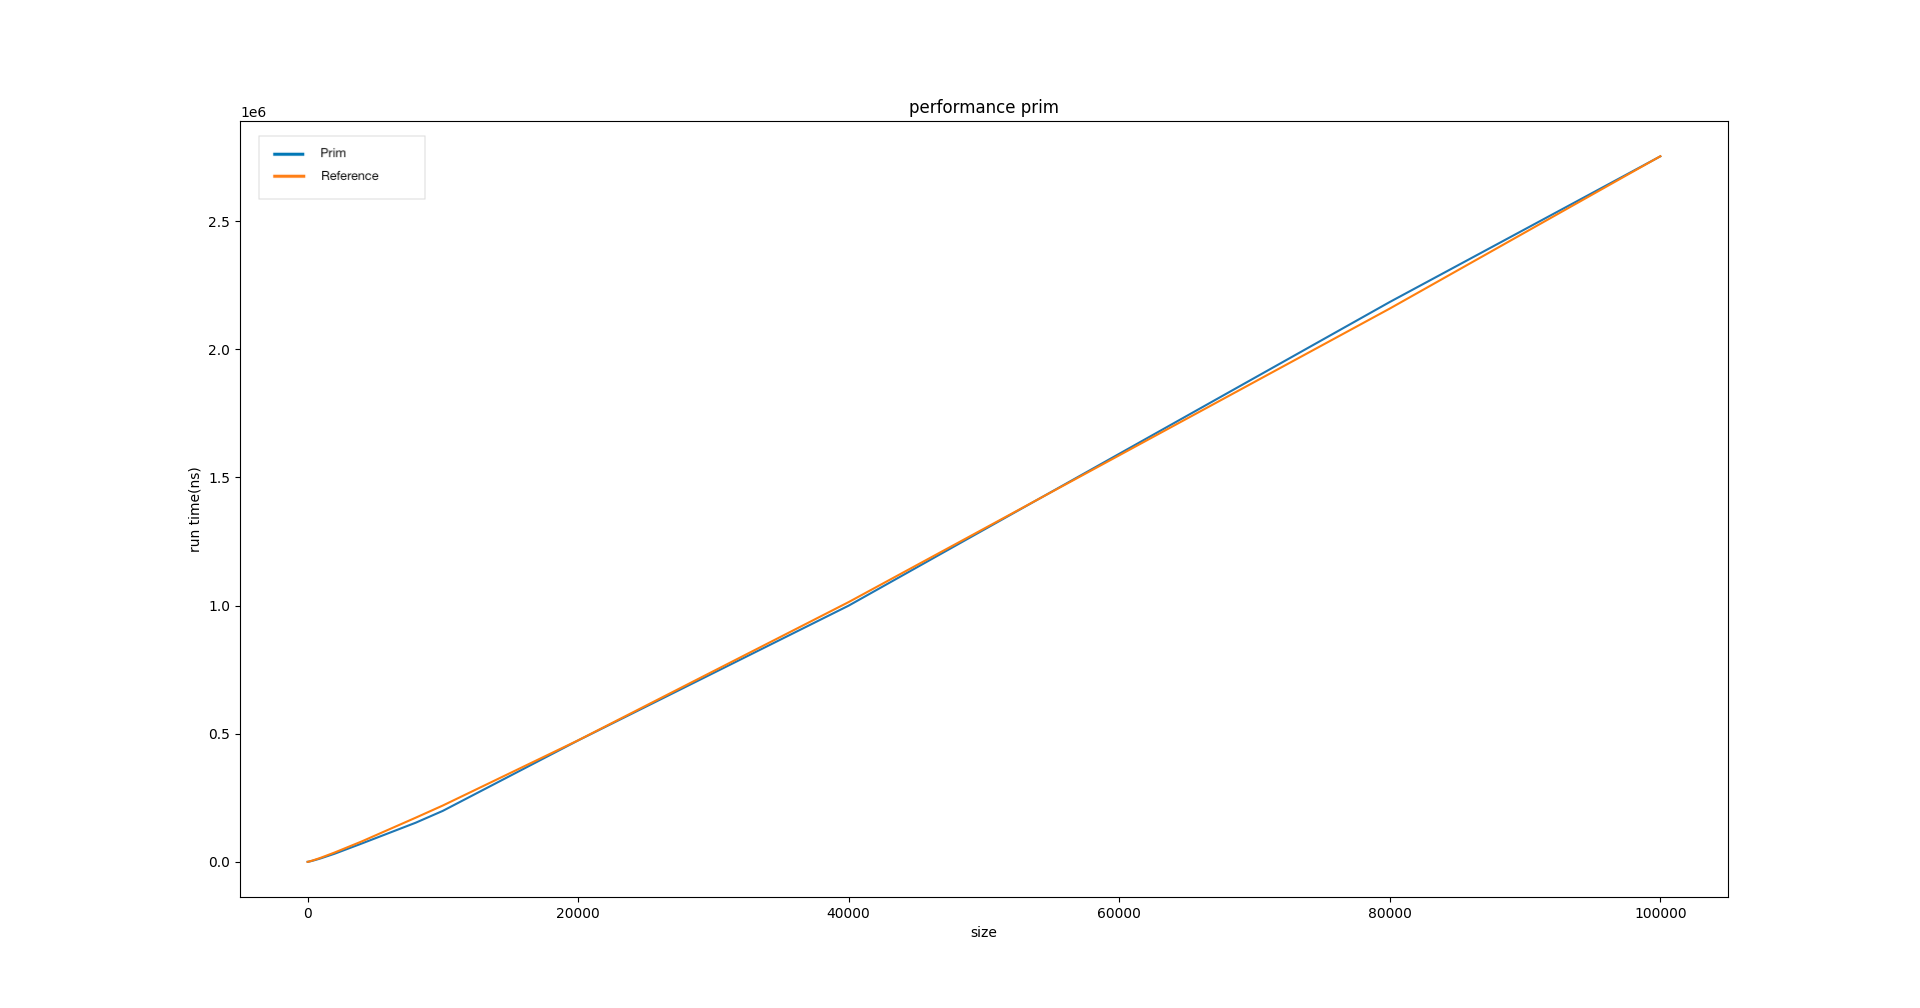
\includegraphics[scale = 0.38]{Fig/primFinale.png}}
    \caption{grafico dei tempi di Prim, in blu si ha il grafico con i tempi teorici moltiplicato per la costante e in arancio il grafico calcolato}
    \label{Prim}
\end{figure}

\newpage

\subsection{Kruskal}
Anche Kruskal, come Prim, ha una complessità di $O(mlogn)$.

\begin{figure}[htbp]
    \centering
    \centerline{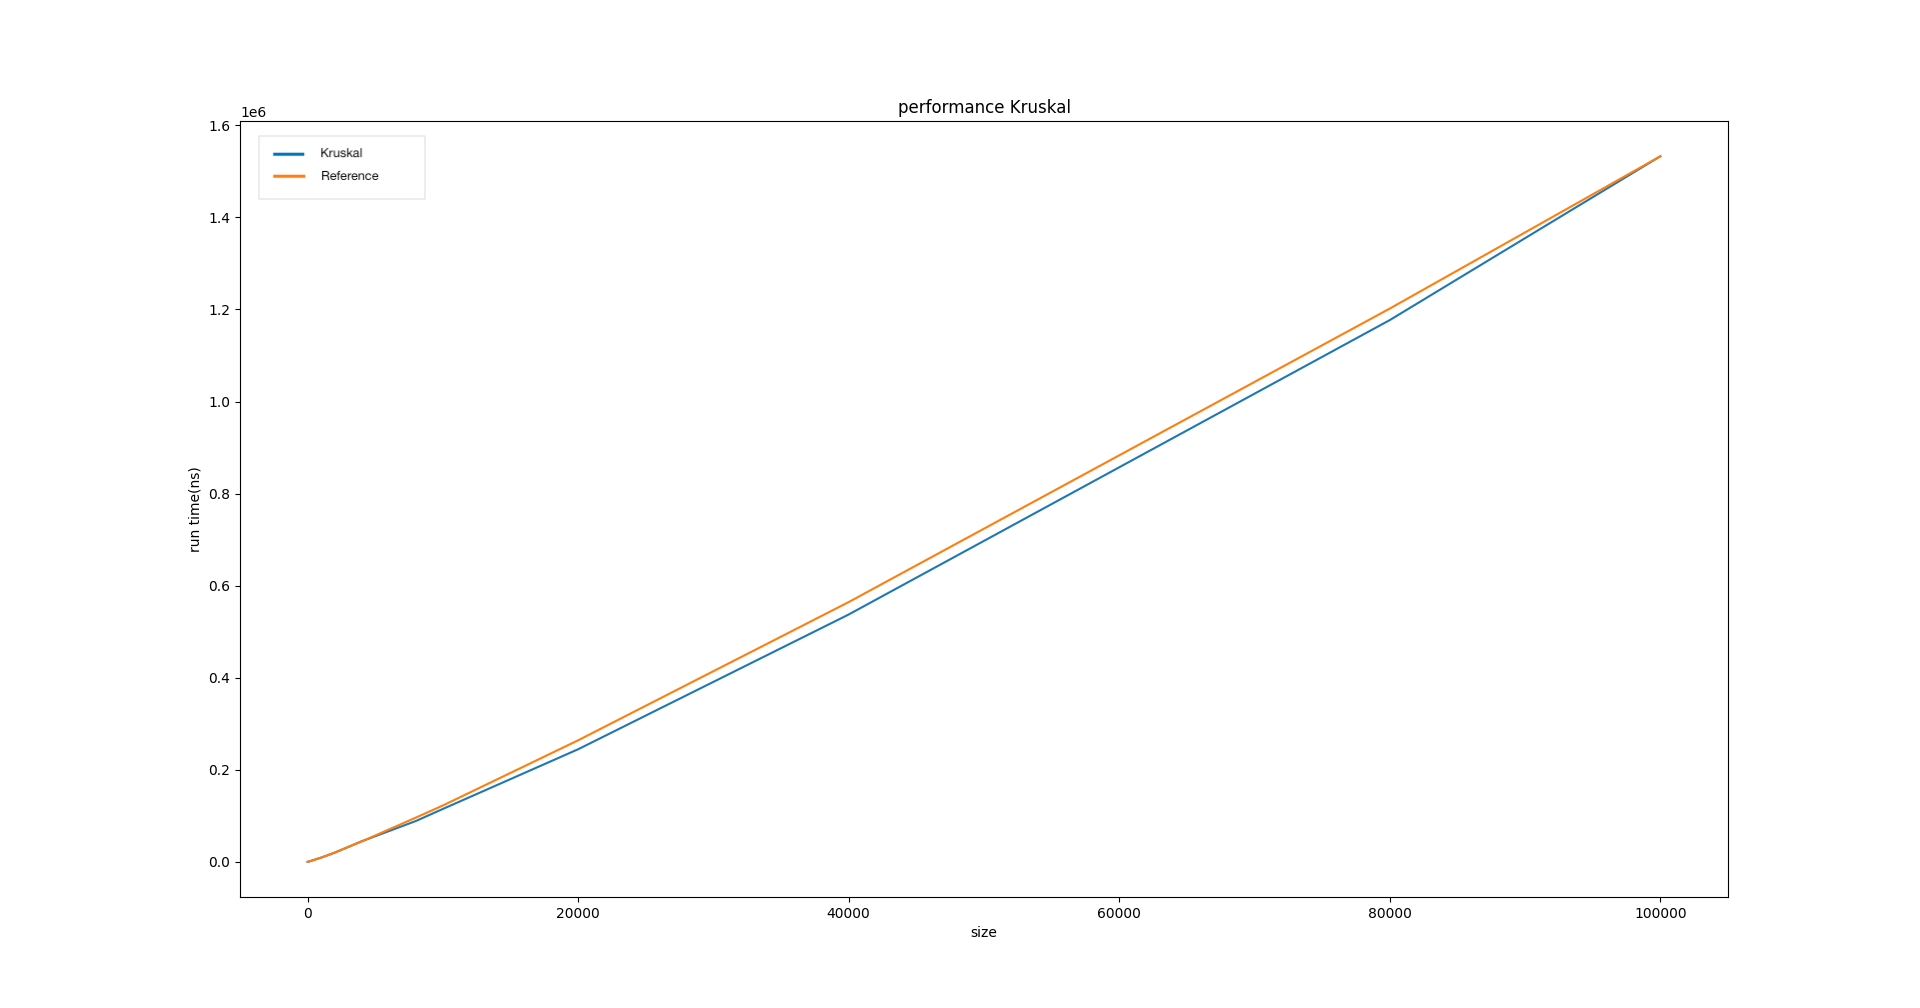
\includegraphics[scale = 0.38]{Fig/KruskalFinale.png}}
    \caption{grafico dei tempi di kruskal,  in blu si ha il grafico con i tempi teorici moltiplicato per la costante e in arancio il grafico calcolato}
    \label{Kruskal}
\end{figure}

\newpage
\subsection{Kruskal naive}
Per quanto riguarda la versione non ottimizzata dell'algoritmo di Kruskal, cioè quella che ad ogni iterazione del ciclo esegue una ricerca in profondità per assicurarsi che il nuovo arco non vada a creare cicli, ha una complessità di $O(mn)$.

Per la versione naive di Kruskal è stata fatta una piccola miglioria. L' algoritmo termina se:
\begin{itemize}
    \item sono stati scorsi tutti i lati del grafo, oppure;
    \item sono stati aggiunti al grafo di copertura minimo n-1 archi, in questo caso viene interrotta l'esecuzione.
\end{itemize}
Dato che la maggior parte dei grafi testati mediamente aveva un numero maggiore di archi rispetto al numero di nodi, grazie alla seconda condizione la costante nascosta all'interno dell'algoritmo si è abbassata. 

\begin{figure}[htbp]
    \centering
    \centerline{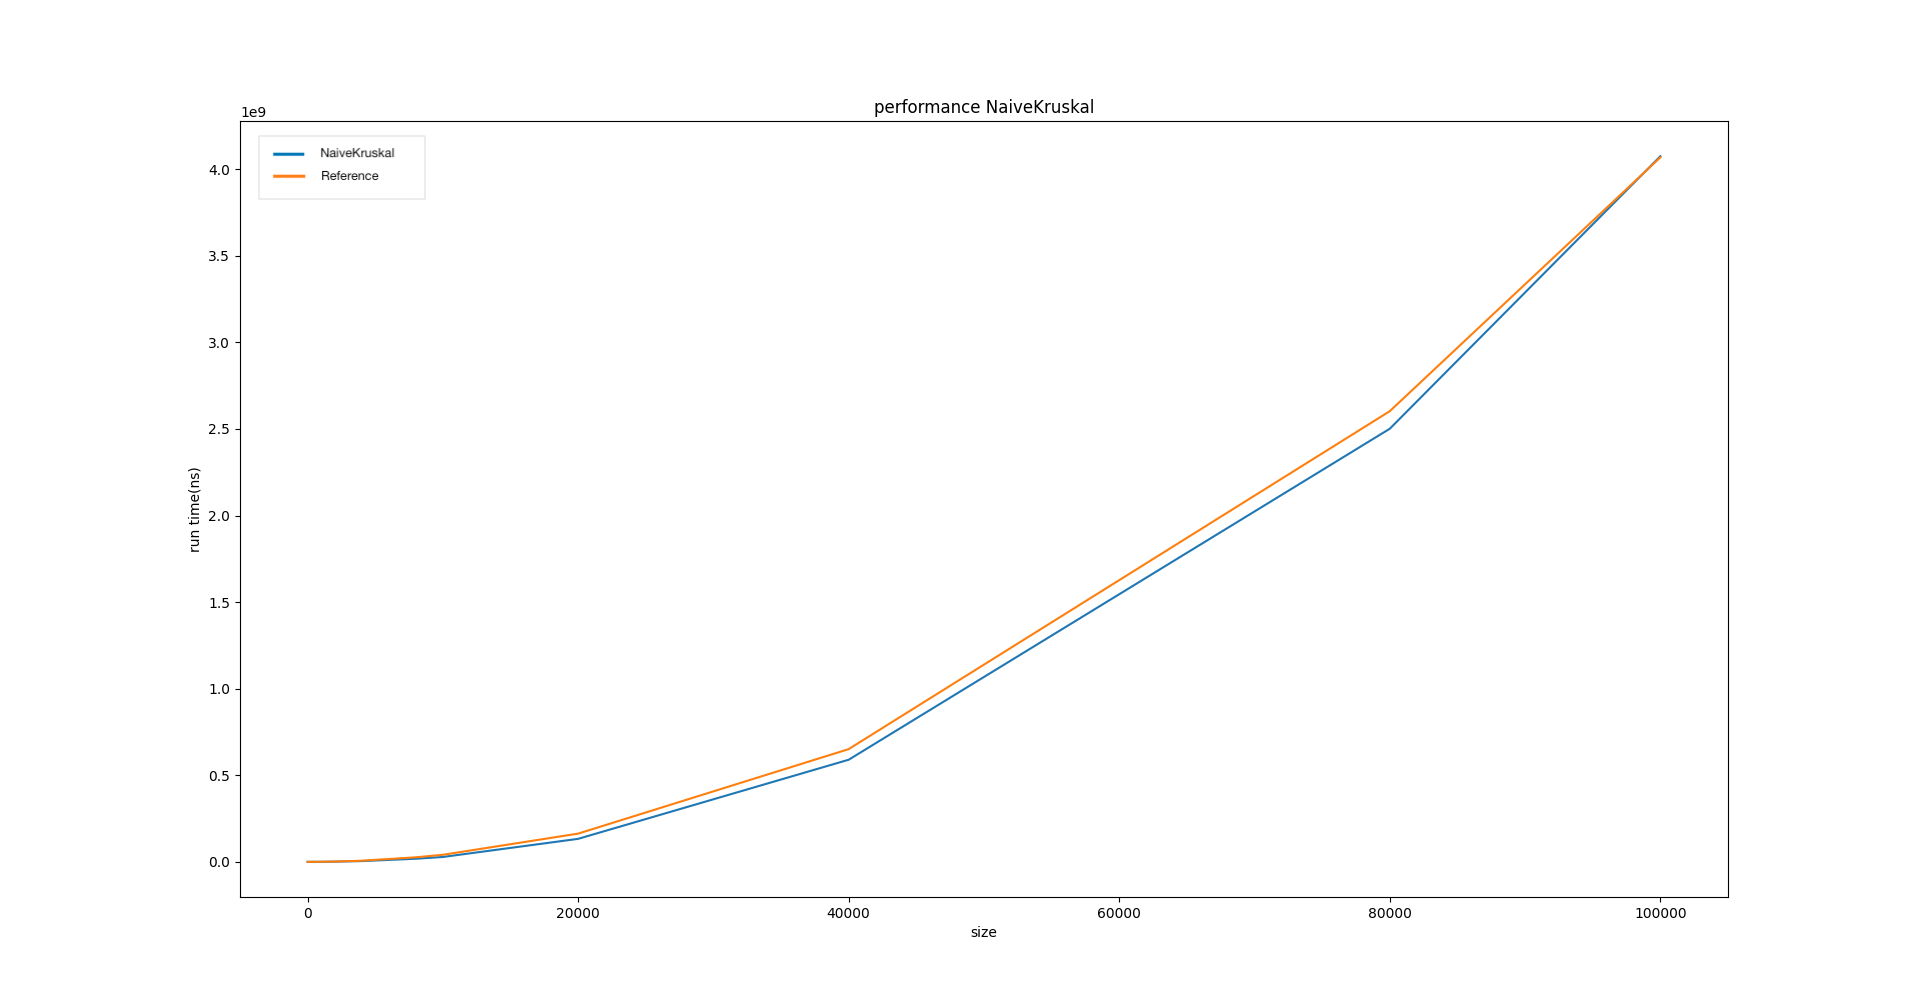
\includegraphics[scale = 0.38]{Fig/NaiveKruskalFinale.png}}
    \caption{grafico dei tempi di Kruskal naive, in blu si ha il grafico con i tempi teorici moltiplicato per la costante e in arancio il grafico calcolato}
    \label{Kruskal naive}
\end{figure}


Come si può notare dai grafici, la curva dei tempi di Prim, Kruskal e Kruskal naive (arancione) va quasi a sovrapporsi ai grafici teorici (blu) moltiplicati per la costante calcolata di ogni algoritmo, questo conferma che l'implementazione rispetta la complessità teorica degli algoritmi.

\newpage
\subsection{Risultati numerici}

Di seguito sono riportate le tabelle con i tempi utilizzati per la costruzione dei grafici sovrastanti. Nell'ordine Prim, Kruskal e KruskalNaive.

\rowcolors{2}{white!80!lightgray!90}{white}
\renewcommand{\arraystretch}{2}
\begin{longtable}[H]{|p{2cm}|p{3cm}|p{2cm}|p{3cm}|} 
\rowcolor{white}
\multicolumn{4}{c}{Continua alla pagina seguente...}
\endfoot
\rowcolor{white}
\caption{tabella riassuntiva di Prim}
\label{tab:tabellaPrim}
\endlastfoot
    \hline
    \rowcolor{lightgray}
    \textbf{n\_nodi} & \textbf{times} & \textbf{costant} & \textbf{ratio}\\ \hline\hline  \endhead
    10	&	38.0	&		1.535	&	None \\ \hline
    20	&	100.0	&		1.309	&	2.632 \\ \hline
    40	&	260.0	&		1.355 &		2.6     \\ \hline
    80	&	619.0	&		1.329 &		2.381  \\ \hline
    100	&	835.0	&		1.358 &		1.349 \\ \hline
    200	&	2021.0	&		1.423 &		2.42 \\ \hline
    400	&	4741.0	&		1.492 &		2.346 \\ \hline
    800	&	10747.0	&		1.515 &		2.267 \\ \hline
    1000 &	14005.0	&		1.534 &		1.303 \\ \hline
    2000 &	31601.0	&		1.557 &		2.256 \\ \hline
    4000 &	71375.0	&	    1.61 &		2.259 \\ \hline
    8000 &	152772.0 &		1.589 &		2.14 \\ \hline
    10000 &	198903.0 &		1.623 &		1.302 \\ \hline
    20000 &	473662.0 &		1.791 &		2.381 \\ \hline
    40000 &	999872.0 &		1.768 &		2.111 \\ \hline
    80000 &	2184898.0 &		1.814 &		2.185 \\ \hline
    100000 &	2753401.0 &	1.793 &		1.26 \\ \hline
\end{longtable}

\newpage

\rowcolors{2}{white!80!lightgray!90}{white}
\renewcommand{\arraystretch}{2}
\begin{longtable}[H]{|p{2cm}|p{3cm}|p{2cm}|p{3cm}|} 
    \rowcolor{white}
\multicolumn{4}{c}{Continua alla pagina seguente...}
\endfoot
\rowcolor{white}
\caption{tabella riassuntiva di Kruskal}
\label{tab:tabellaKruskal}
\endlastfoot
\hline
    \rowcolor{lightgray}
    \textbf{n\_nodi} & \textbf{times} & \textbf{costant} & \textbf{ratio} \\ \hline\hline
    \endhead
    10	&	    46.0	&		1.858 &		None \\ \hline
    20	&	    113.0	&		1.479 &		2.457 \\ \hline
    40	&	    238.0	&		1.241 &		2.106 \\ \hline
    80	&	    522.0	&		1.121 &		2.193 \\ \hline
    100	&	    650.0	&		1.057 &		1.245 \\ \hline
    200	&	    1593.0	&		1.122 &		2.451 \\ \hline
    400	&	    3486.0	&		1.097 &		2.188 \\ \hline
    800	&	    7315.0	&		1.031 &		2.098 \\ \hline
    1000 &	    9082.0	&		0.995 &		1.242 \\ \hline
    2000 &	    19697.0	&		0.97  &  	2.169 \\ \hline
    4000 &	    44597.0	&	    1.006 &		2.264 \\ \hline
    8000 &		88609.0	&	    0.922 &		1.987 \\ \hline
    10000 &		114837.0 &		0.937 &		1.296 \\ \hline
    20000 &		244539.0 &		0.924 &		2.129 \\ \hline
    40000 &		537266.0 &		0.95 &		2.197 \\ \hline
    80000 &		1176867.0 &		0.977 &	    2.19 \\ \hline
    100000 &	1532773.0 &		0.998 &	    1.302 \\ \hline
\end{longtable}

\newpage
\rowcolors{2}{white!80!lightgray!90}{white}
\renewcommand{\arraystretch}{2}
\begin{longtable}[H]{|p{2cm}|p{3cm}|p{2cm}|p{3cm}|} 
    \rowcolor{white}
\multicolumn{4}{c}{Continua alla pagina seguente...}
\endfoot
\rowcolor{white}
\caption{tabella riassuntiva di Kruskal naive}
\label{tab:tabellaKriskalNaive}
\endlastfoot
\hline
    \rowcolor{lightgray}
    \textbf{n\_nodi} & \textbf{times} & \textbf{costant} & \textbf{ratio} \\ \hline\hline
    \endhead
    10	&	72.0		&	0.67	&	None \\ \hline
    20	&	238.0		&	0.467	&	3.306 \\ \hline
    40	&	583.0		&	0.28 &		2.45 \\ \hline
    80	&	2485.0		&	0.292 &		4.262 \\ \hline
    100	&	3034.0		&	0.227   &	1.221 \\ \hline
    200	&	11917.0		&	0.222	&	3.928 \\ \hline
    400	&	42721.0		&	0.201	&	3.585 \\ \hline
    800	&	166700.0	&	0.196	&   3.902 \\ \hline
    1000 &	262169.0	&	0.198	&   1.573 \\ \hline
    2000 &	1099545.0	&	0.206	&   4.194 \\ \hline
    4000 &	4371607.0	&	0.204 &		3.976 \\ \hline
    8000 &	17944643.0	&	0.21 &		4.105 \\ \hline
    10000 &	28077773.0	&	0.211 &		1.565 \\ \hline
    20000 &	132740246.0	&	0.248 &		4.728 \\ \hline
    40000 &	589607712.0	&	0.276 &		4.442 \\ \hline
    80000 &	2501403023.0 &	0.293 &		4.242 \\ \hline
    100000 &	4075177518.0 &	0.305 &		1.629 \\ \hline
\end{longtable}

Come si può notare dalle tabelle che riassumono i risultati per ogni algoritmo, anche il ratio calcolato corrisponde a quello voluto. Infatti per quanto riguarda il ratio di Prim e Kruskal ($\sim 2,2$) \footnote{il ratio considerato, così come la costante per calcolare il grafico teorica, è quello corrispondente all'ultima istanza (100000)} sono quasi equivalenti e corrispondono al ratio teorico $2m*log(2n) / m*log(n)$.
Equivalentemente lo stesso discorso vale per Kruskal naive dove il ratio (4,4) corrisponde a circa il ratio teorico $2m*2n/m*n$



\newpage
\section{Conclusioni}
\label{conlusioni}

Dal grafico in Figura 4, e soprattutto dal grafico in Figura 5, si può notare che generalmente Kruskal è più veloce rispetto a Prim in quasi tutte le istanze, e quindi quasi sempre più efficiente. Questo è dovuto al fatto che Kruskal ha in genere una costante nascosta più piccola rispetto a Prim, come si può notare nella tabella 1 e 2.
Anche se questo non è vero per tutte le istanze, infatti Prim si comporta leggermente meglio con le istanze di bassa dimensionalità (n\_nodi <= 20).

\begin{figure}[htbp]
    \centering
    \centerline{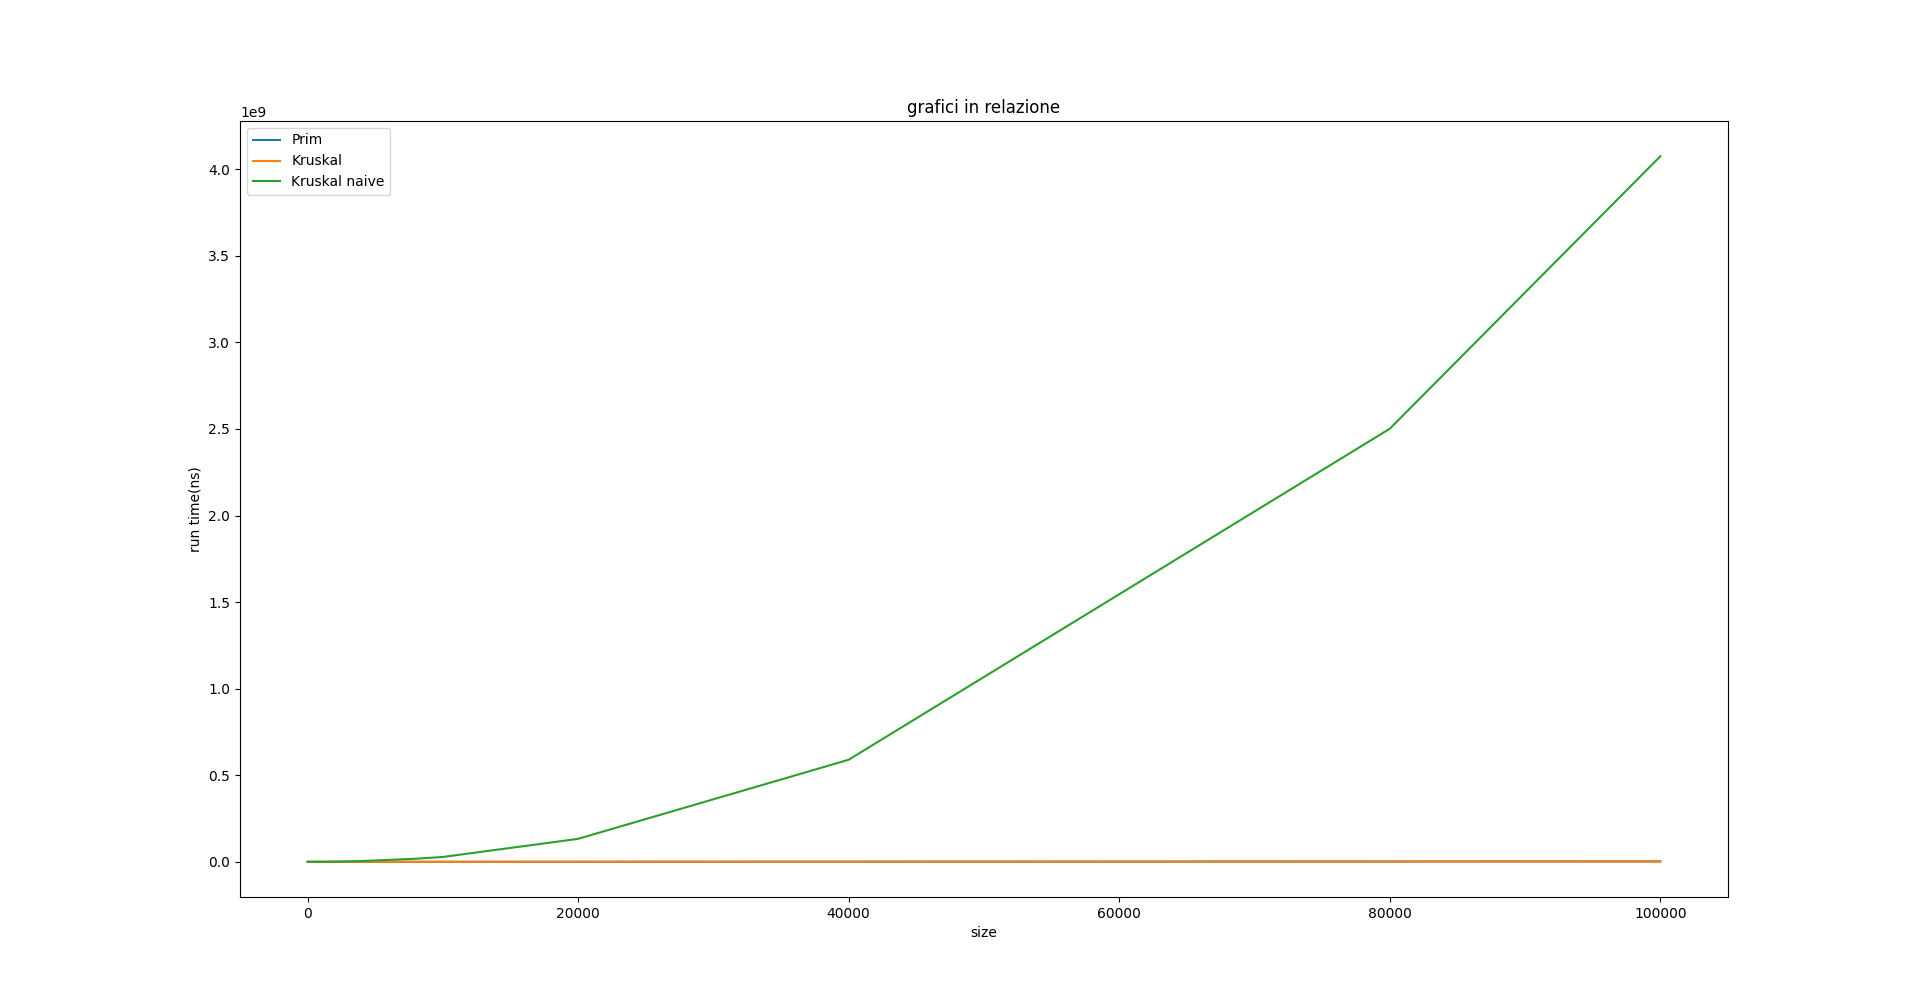
\includegraphics[scale = 0.38]{Fig/graficiRelazione.png}}
    \caption{grafico che mostra il confronto tra i 3 algoritmi: Naive Kruskal(verde), Kruskal(arancione), Prim(blu). Come si può notare dal grafico in figura 4, Kruskal naive cresce molto più velocemnte rispetto a Prim e Kruskal}
\end{figure}

\newpage

\begin{figure}[htbp]
    \centering
    \centerline{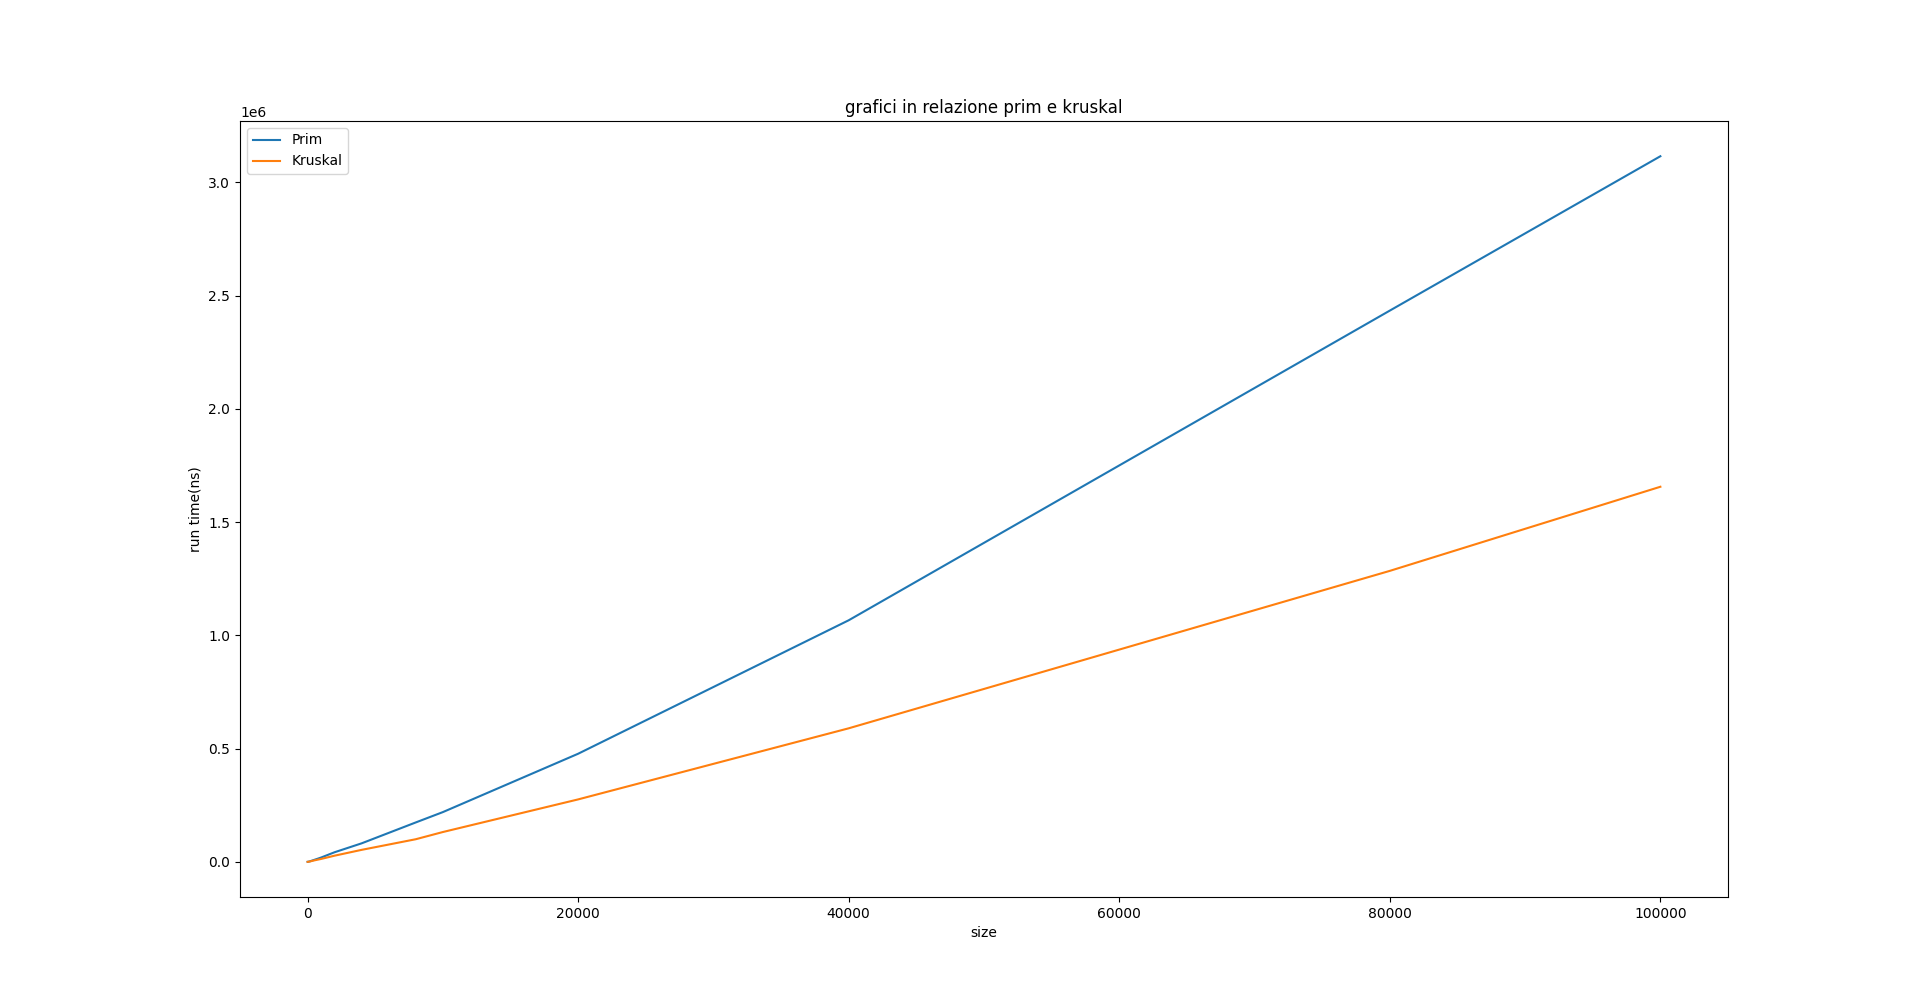
\includegraphics[scale = 0.38]{Fig/primkruskalrelazione.png}}
    \caption{grafico che mostra il confronto tra Prim(blu) e Kruskal(arancione)}
\end{figure}

\newpage

\subsection{Tabella pesi}
\label{tabellaPesi}

Di seguito viene riportata la tabella del calcolo dei pesi per ogni istanza divisi in base agli algoritmi. È possibile notare l'uguaglianza tra i pesi risultanti.
Con n\_nodi e n\_archi ci si riferisce al numero di nodi e al numero di archi del grafo originale, e non dell'albero di copertura minimo calcolato. 

\rowcolors{2}{white!80!lightgray!90}{white}
\renewcommand{\arraystretch}{2}
\begin{longtable}[H]{|p{1.5cm}|p{1.5cm}|p{2cm}|p{3cm}|p{4cm}|} 
    \rowcolor{white}
    \multicolumn{5}{c}{Continua alla pagina seguente...}
    \endfoot
    \rowcolor{white}
    \endlastfoot
    \hline
    \rowcolor{lightgray}
    \textbf{n\_nodi} & \textbf{n\_archi} & \textbf{peso Prim} & \textbf{peso Kruskal} & \textbf{peso Kruskal naive} \\ \hline\hline
    \endhead
    10 & 9 & 29316 & 29316 & 29316 \\ \hline
    10 & 10 & 25217 & 25217 & 25217 \\ \hline
    10 & 11 & 16940 & 16940 & 16940 \\ \hline
    10 & 13 & -44448 & -44448 & -44448 \\ \hline
    20 & 24 & -32021 & -32021 & -32021 \\ \hline 
    20 & 24 & 25130 & 25130 & 25130 \\ \hline
    20 & 26 & -37205 & -37205 & -37205 \\ \hline
    20 & 28 & -41693 & -41693 & -41693 \\ \hline
    40 & 50 & -31929 & -31929 & -31929 \\ \hline
    40 & 50 & -79570 & -79570 & -79570 \\ \hline
    40 & 52 & -79741 & -79741 & -79741 \\ \hline
    40 & 56 & -114203 & -114203 & -114203 \\ \hline
    80 & 99 & -198094 & -198094 & -198094 \\ \hline
    80 & 104 & -110571 & -110571 & -110571 \\ \hline
    80 & 108 & -139926 & -139926 & -139926 \\ \hline
    80 & 114 & -233320 & -233320 & -233320 \\ \hline
    100 & 129 & -271743 & -271743 & -271743 \\ \hline
    100 & 132 & -229506 & -229506 & -229506 \\ \hline
    100 & 136 & -141960 & -141960 & -141960 \\ \hline
    100 & 137 & -288906 & -288906 & -288906 \\ \hline
    200 & 267 & -393278 & -393278 & -393278 \\ \hline
    200 & 267 & -510185 & -510185 & -510185 \\ \hline
    200 & 269 & -444357 & -444357 & -444357 \\ \hline
    200 & 269 & -515136 & -515136 & -515136 \\ \hline
    400 & 518 & -788168 & -788168 & -788168 \\ \hline
    400 & 526 & -733645 & -733645 & -733645 \\ \hline
    400 & 538 & -895704 & -895704 & -895704 \\ \hline
    400 & 540 & -1119906 & -1119906 & -1119906 \\ \hline
    800 & 1049 & -1652119 & -1652119 & -1652119 \\ \hline 
    800 & 1058 & -1578294 & -1578294 & -1578294 \\ \hline 
    800 & 1063 & -1541291 & -1541291 & -1541291 \\ \hline
    800 & 1076 & -1664316 & -1664316 & -1664316 \\ \hline
    1000 & 1300 & -2089013 & -2089013 & -2089013 \\ \hline
    1000 & 1313 & -1934208 & -1934208 & -1934208 \\ \hline
    1000 & 1328 & -2229428 & -2229428 & -2229428 \\ \hline
    1000 & 1344 & -2356163 & -2356163 & -2356163 \\ \hline
    2000 & 2652 & -4717250 & -4717250 & -4717250 \\ \hline
    2000 & 2654 & -4739387 & -4739387 & -4739387 \\ \hline 
    2000 & 2677 & -4537267 & -4537267 & -4537267 \\ \hline 
    2000 & 2699 & -4811598 & -4811598 & -4811598 \\ \hline 
    4000 & 5315 & -9314968 & -9314968 & -9314968 \\ \hline
    4000 & 5340 & -9845767 & -9845767 & -9845767 \\ \hline
    4000 & 5360 & -8722212 & -8722212 & -8722212 \\ \hline
    4000 & 5368 & -8681447 & -8681447 & -8681447 \\ \hline 
    8000 & 10662 & -18741474 & -18741474 & -18741474 \\ \hline  
    8000 & 10670 & -18798446 & -18798446 & -18798446 \\ \hline  
    8000 & 10705 & -17844628 & -17844628 & -17844628 \\ \hline
    8000 & 10757 & -18178610 & -18178610 & -18178610 \\ \hline  
    10000 & 13287 & -22581384 & -22581384 & -22581384 \\ \hline
    10000 & 13301 & -22079522 & -22079522 & -22079522 \\ \hline
    10000 & 13311 & -22606313 & -22606313 & -22606313 \\ \hline
    10000 & 13340 & -22338561 & -22338561 & -22338561 \\ \hline 
    20000 & 26667 & -45962292 & -45962292 & -45962292 \\ \hline
    20000 & 26670 & -46418161 & -46418161 & -46418161 \\ \hline
    20000 & 26673 & -47854708 & -47854708 & -47854708 \\ \hline
    20000 & 26826 & -45195405 & -45195405 & -45195405 \\ \hline
    40000 & 53242 & -88771991 & -88771991 & -88771991 \\ \hline
    40000 & 53319 & -93017025 & -93017025 & -93017025 \\ \hline
    40000 & 53415 & -92003321 & -92003321 & -92003321 \\ \hline
    40000 & 53446 & -94397064 & -94397064 & -94397064 \\ \hline
    80000 & 106554 & -180793224 & -180793224 & -180793224 \\ \hline 
    80000 & 106586 & -182065015 & -182065015 & -182065015 \\ \hline 
    80000 & 106633 & -185997521 & -185997521 & -185997521 \\ \hline
    80000 & 106914 & -186834082 & -186834082 & -186834082 \\ \hline
    100000 & 133214 & -230168572 & -230168572 & -230168572 \\ \hline
    100000 & 133395 & -230698391 & -230698391 & -230698391 \\ \hline
    100000 & 133463 & -231011693 & -231011693 & -231011693 \\ \hline
    100000 & 133524 & -231393935 & -231393935 & -231393935  \\ \hline
\end{longtable}
\newpage
\subsection{Tabella tempi}
\label{tabellaTempi}
Di seguito invece è riportata la tabella con i tempi di esecuzione per ogni algoritmo e per ogni istanza. Si può notare come nelle prime istanze Prim performa meglio rispetto a Kruskal, mentre nelle istanze successive ha sempre un tempo di esecuzione maggiore.


\rowcolors{2}{white!80!lightgray!90}{white}
\renewcommand{\arraystretch}{2}
\begin{longtable}[H]{|p{1.5cm}|p{1.5cm}|p{2cm}|p{2cm}|p{3cm}|p{3cm}|} 
    \rowcolor{white}
    \multicolumn{6}{c}{Continua alla pagina seguente...}
    \endfoot
    \rowcolor{white}
    \endlastfoot
    \hline
    \rowcolor{lightgray}
    \textbf{n\_nodi} & \textbf{n\_archi} & \textbf{Prim} & \textbf{Kruskal} & \textbf{Kruskal naive} & \textbf{alg. migliore}\\ \hline\hline
    \endhead
    10 & 9 & 37.0 & 43.0 & 66.0 & Prim : 37.0 \\ \hline
    10 & 10 & 34.0 & 45.0 & 78.0 & Prim : 34.0 \\ \hline
    10 & 11 & 42.0 & 46.0 & 64.0 & Prim : 42.0 \\ \hline
    10 & 13 & 37.0 & 50.0 & 79.0 & Prim : 37.0 \\ \hline
    20 & 24 & 98.0 & 101.0 & 207.0 & Prim : 98.0 \\ \hline
    20 & 24 & 92.0 & 109.0 & 236.0 & Prim : 92.0 \\ \hline
    20 & 26 & 104.0 & 111.0 & 213.0 & Prim : 104.0 \\ \hline
    20 & 28 & 105.0 & 132.0 & 294.0 & Prim : 105.0 \\ \hline
    40 & 50 & 244.0 & 230.0 & 606.0 & Kruskal : 230.0 \\ \hline
    40 & 50 & 282.0 & 236.0 & 592.0 & Kruskal : 236.0 \\ \hline
    40 & 52 & 249.0 & 244.0 & 545.0 & Kruskal : 244.0 \\ \hline
    40 & 56 & 264.0 & 243.0 & 587.0 & Kruskal : 243.0 \\ \hline
    80 & 99 & 603.0 & 499.0 & 2441.0 & Kruskal : 499.0 \\ \hline
    80 & 104 & 575.0 & 526.0 & 2178.0 & Kruskal : 526.0 \\ \hline
    80 & 108 & 639.0 & 521.0 & 2367.0 & Kruskal : 521.0 \\ \hline
    80 & 114 & 659.0 & 540.0 & 2956.0 & Kruskal : 540.0 \\ \hline
    100 & 129 & 810.0 & 642.0 & 2756.0 & Kruskal : 642.0 \\ \hline
    100 & 132 & 847.0 & 641.0 & 3031.0 & Kruskal : 641.0 \\ \hline
    100 & 136 & 814.0 & 673.0 & 3831.0 & Kruskal : 673.0 \\ \hline
    100 & 137 & 869.0 & 644.0 & 2518.0 & Kruskal : 644.0 \\ \hline
    200 & 267 & 2051.0 & 1604.0 & 13963.0 & Kruskal : 1604.0 \\ \hline 
    200 & 267 & 2011.0 & 1594.0 & 12516.0 & Kruskal : 1594.0 \\ \hline 
    200 & 269 & 2075.0 & 1589.0 & 10441.0 & Kruskal : 1589.0 \\ \hline 
    200 & 269 & 1946.0 & 1586.0 & 10749.0 & Kruskal : 1586.0 \\ \hline 
    400 & 518 & 4642.0 & 3274.0 & 36730.0 & Kruskal : 3274.0 \\ \hline 
    400 & 526 & 4814.0 & 3423.0 & 44668.0 & Kruskal : 3423.0 \\ \hline 
    400 & 538 & 4760.0 & 3872.0 & 41741.0 & Kruskal : 3872.0 \\ \hline 
    400 & 540 & 4748.0 & 3377.0 & 47742.0 & Kruskal : 3377.0 \\ \hline 
    800 & 1049 & 10668.0 & 7820.0 & 169127.0 & Kruskal : 7820.0 \\ \hline
    800 & 1058 & 10675.0 & 6827.0 & 164728.0 & Kruskal : 6827.0 \\ \hline
    800 & 1063 & 10913.0 & 7739.0 & 168908.0 & Kruskal : 7739.0 \\ \hline
    800 & 1076 & 10730.0 & 6873.0 & 164036.0 & Kruskal : 6873.0 \\ \hline
    1000 & 1300 & 14330.0 & 9562.0 & 248674.0 & Kruskal : 9562.0 \\ \hline
    1000 & 1313 & 13637.0 & 8709.0 & 271322.0 & Kruskal : 8709.0 \\ \hline
    1000 & 1328 & 13929.0 & 9082.0 & 269150.0 & Kruskal : 9082.0 \\ \hline
    1000 & 1344 & 14125.0 & 8976.0 & 259530.0 & Kruskal : 8976.0 \\ \hline
    2000 & 2652 & 30916.0 & 18345.0 & 1059458.0 & Kruskal : 18345.0 \\ \hline 
    2000 & 2654 & 31651.0 & 18992.0 & 1075133.0 & Kruskal : 18992.0 \\ \hline 
    2000 & 2677 & 32052.0 & 20291.0 & 1113125.0 & Kruskal : 20291.0 \\ \hline 
    2000 & 2699 & 31787.0 & 21161.0 & 1150464.0 & Kruskal : 21161.0 \\ \hline 
    4000 & 5315 & 71565.0 & 43781.0 & 4362490.0 & Kruskal : 43781.0 \\ \hline 
    4000 & 5340 & 70825.0 & 45548.0 & 4164992.0 & Kruskal : 45548.0 \\ \hline 
    4000 & 5360 & 70934.0 & 44696.0 & 4351926.0 & Kruskal : 44696.0 \\ \hline 
    4000 & 5368 & 72175.0 & 44362.0 & 4607022.0 & Kruskal : 44362.0 \\ \hline 
    8000 & 10662 & 153353.0 & 87139.0 & 17275593.0 & Kruskal : 87139.0 \\ \hline
    8000 & 10670 & 150470.0 & 87487.0 & 17472939.0 & Kruskal : 87487.0 \\ \hline
    8000 & 10705 & 155038.0 & 90897.0 & 19034256.0 & Kruskal : 90897.0 \\ \hline
    8000 & 10757 & 152228.0 & 88914.0 & 17995782.0 & Kruskal : 88914.0 \\ \hline
    10000 & 13287 & 199069.0 & 114678.0 & 27519384.0 & Kruskal : 114678.0 \\ \hline 
    10000 & 13301 & 198213.0 & 114541.0 & 28212040.0 & Kruskal : 114541.0 \\ \hline 
    10000 & 13311 & 198148.0 & 114831.0 & 28410336.0 & Kruskal : 114831.0 \\ \hline 
    10000 & 13340 & 200183.0 & 115300.0 & 28169334.0 & Kruskal : 115300.0 \\ \hline 
    20000 & 26667 & 460829.0 & 247868.0 & 135050130.0 & Kruskal : 247868.0 \\ \hline
    20000 & 26670 & 466592.0 & 240454.0 & 131505987.0 & Kruskal : 240454.0 \\ \hline
    20000 & 26673 & 461937.0 & 245921.0 & 131375244.0 & Kruskal : 245921.0 \\ \hline
    20000 & 26826 & 505290.0 & 243914.0 & 133029623.0 & Kruskal : 243914.0 \\ \hline
    40000 & 53242 & 1052767.0 & 539613.0 & 582092711.0 & Kruskal : 539613.0 \\ \hline 
    40000 & 53319 & 1017180.0 & 530200.0 & 579462411.0 & Kruskal : 530200.0 \\ \hline 
    40000 & 53415 & 962333.0 & 541707.0 & 602520927.0 & Kruskal : 541707.0 \\ \hline 
    40000 & 53446 & 967208.0 & 537543.0 & 594354801.0 & Kruskal : 537543.0 \\ \hline 
    80000 & 106554 & 2246350.0 & 1180804.0 & 2484800866.0 & Kruskal : 1180804.0 \\ \hline
    80000 & 106586 & 2131476.0 & 1175085.0 & 2497156786.0 & Kruskal : 1175085.0 \\ \hline
    80000 & 106633 & 2148715.0 & 1172859.0 & 2503001407.0 & Kruskal : 1172859.0 \\ \hline
    80000 & 106914 & 2213052.0 & 1178719.0 & 2520653034.0 & Kruskal : 1178719.0 \\ \hline
    100000 & 133214 & 2769982.0 & 1537615.0 & 4041731255.0 & Kruskal : 1537615.0 \\ \hline 
    100000 & 133395 & 2761894.0 & 1533403.0 & 4099202631.0 & Kruskal : 1533403.0 \\ \hline 
    100000 & 133463 & 2738139.0 & 1531136.0 & 4041570425.0 & Kruskal : 1531136.0 \\ \hline 
    100000 & 133524 & 2743588.0 & 1528937.0 & 4118205760.0 & Kruskal : 1528937.0 \\ \hline 
\end{longtable}












\newpage
%%% Appendici %%%

\end{document}